\documentclass{article}
\usepackage[utf8]{inputenc}
\usepackage[english]{babel}
\usepackage{graphicx}
\usepackage{color}
\usepackage{amsfonts}
\usepackage{amssymb}
\usepackage{enumitem}

\usepackage[a4paper, total={6in, 8in}]{geometry}




\def\warning#1{\color{red} #1 \color{black}}
\def\note#1{\color{cyan} #1 \color{black}}
\def\circled#1{\raisebox{.5pt}{\textcircled{\raisebox{-.9pt} {#1}}}}

\def\solution#1{\color{cyan}\textit{Oplossing: #1}\color{black}}
\graphicspath{{./img/}}

\begin{document}

\title{Examen Discrete Wiskunde 20 augustus 2018}
\date{}
\author{}
\maketitle

\note{Het percentageteken voor elke vraag wijst op de relatieve score van die vraag}

\begin{enumerate}
\item{\note{10\%} Bereken eerst de kleinste primitieve wortel $\omega$ in ($\mathbb{Z}_{9001}, \cdot)$. Bepaal hierna voor elke geheel getal $\alpha < \omega$ de orde van $\alpha$. Een oplossing louter gebaseerd op het berekenen van opeenvolgende machten van $\alpha$ wordt als waardeloos beschouwd.}

\item{\note{6\%} Produceer een Hamiltoncyclus in $Q_9$. Wat is de lengte van het pad tussen de knopen met identificatie $010101010$ en $101010101$?}

\item {Beschouw het veld $F_{16}$ en de elliptische kromme E: $y^2+xy = x^3 + \circled{3}x^2 + \circled{5} $ over dit veld. De irreducibele veelterm is $\mu = x^4 + x + 1$ en de primitieve wortel $\omega = x$. Gebruik de onderstaande groepstabel: 
\begin{center}
 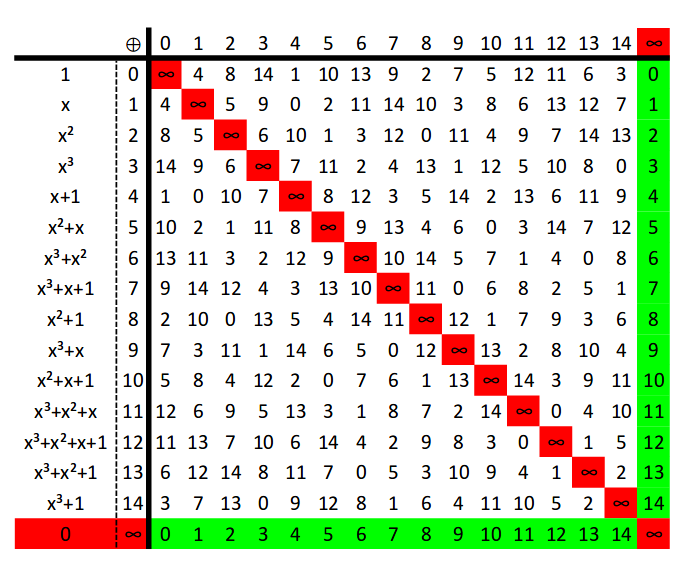
\includegraphics[width=\linewidth]{groepstabel}
\end{center}

\item{
    \begin{itemize}[label={}]
    
    \item \note{12\%} Het punt $A(x + 1, x^3)$ is één van de punten van de elliptische kromme E. Bepaal alle andere punten en duid hierbij aan welke inversen zijn van elkaar. Hoeveel punten heeft deze elliptische kromme?

    \item \note{8\%} Bereken 2A, 4A en 8A en identificeer het resultaat met één van de hiervoor gevonden punten.
    
    
    \item \note{8\%} Bereken de overige veelvouden van A, tot je hetzij het neutrale element, hetzij het punt dat zijn eigen inverse is bekomt. Bepaal hieruit de structuur van de overeenkomstige groep. Is de groep cyclisch en zo ja, met hoeveel primitieve elementen. 


      \end{itemize}}
}
  \item {
    \begin{itemize}[label={}]
        \item \note{8\%} Bepaal het multiplicatieve inverse van $x^4 + x^2 + 4$ int het veld $F_{3125}$ met betrekking tot $x^5 + x^4 + 4$ als irreducibele veelterm.
        \item \note{6\%} Bereken, met behulp van het antwoord van de vorige vraag, $\omega^{2011}$
    \end{itemize}
  
  }
  \item {\note{12\%} \warning{Hexiamonds plaatsen zodat elke spijker slechts door 1 hexiamond gaat en het grid moet volledig opgevuld zijn, het grid is een hexagon opgedeeld in driehoeken}}    
  
  \item {\note{10\%}}Ter herinnering kan je in de folder \textit{groepstabellen} enkele groepen terugvinden van orde 4 en 6. Bepaal volgende (semi)-directe producten:
        \begin{itemize}
         \item $C_4 \rtimes C_6$
         \item $S_3 \rtimes $
         \item $C_6 \rtimes C_4$
         \item $C_4 \times C_6$
        \end{itemize}


                    
                    

  \item {\begin{itemize}
      \item {\note{18\%} Bepaal de cykelindex om de facetten van een rombische dodecaëder (Rhombic dodecahedron), waarbij zowel rotaties als spiegelingen in beschouwing worden genomen. Je kan deze figuur manipuleren door het programma Antiview op te starten met als enige argument \textit{rd}.
        }
      \item {\note{6\%} Hoeveel configuraties zijn er mogelijk waarbij er 2 kleuren 6 maal gebruikt worden. Hoeveel van deze configuraties zijn een spiegelbeeld van elkaar?

      \item {\note{6\%} Hoeveel configuraties zijn er mogelijk waarbij er 3 kleuren 4 maal gebruikt worden. Hoeveel van deze configuraties zijn een spiegelbeeld van elkaar?}
      }
      \end{itemize}}
\end{enumerate}



\end{document}


% green 147 BLUE 240
